% !TEX root = ../main.tex
%\vspace{-0.1in}
\section{LoCo: Local Contrastive Representation Learning}
\label{sec:method}
In this section, we will introduce our approach to close the gap between local contrastive learning and state-of-the-art end-to-end learning. 

\begin{figure}[t]
\vspace{-0.2in}
  \centering
  \iflatexml
  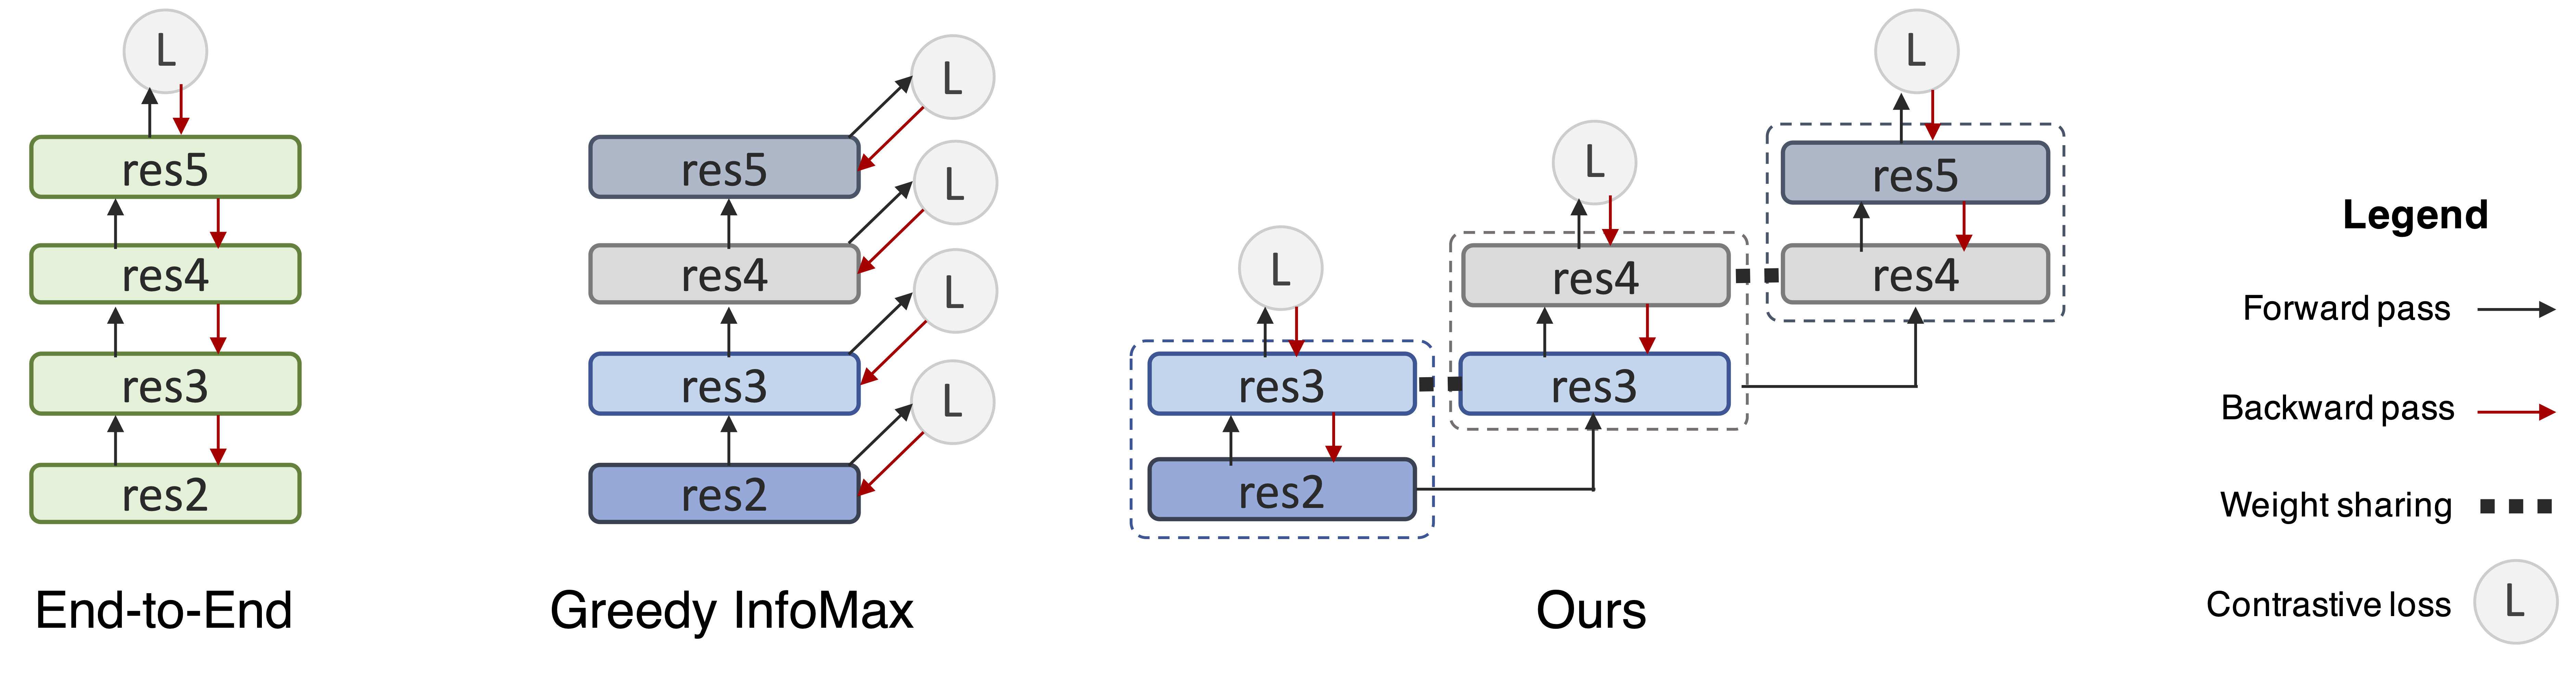
\includegraphics[width=6\textwidth,clip]{figures/mainfig_res.png}
  \else
  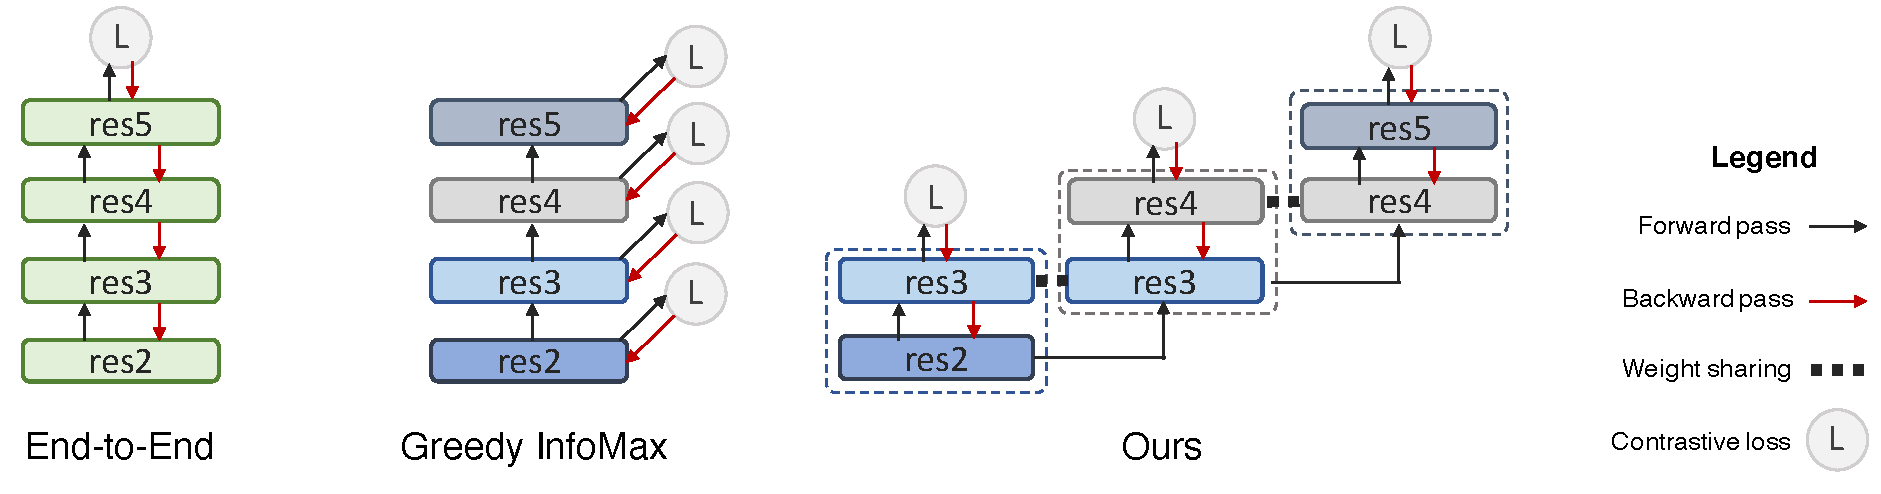
\includegraphics[width=0.98\textwidth,clip]{figures/mainfig_res.pdf}
  \fi
  \caption{Comparison between End-to-End, Greedy InfoMax (GIM) and {\ours}}
  \label{fig:prev_model}
\vspace{-0.1in}
\end{figure}

In the left part of Fig.~\ref{fig:prev_model}, we show a regular end-to-end network using
backpropagation, where each rectangle denotes a downsample stage. In ResNet-50, they are {\em
conv1+res2}, {\em res3}, {\em res4}, {\em res5}. In the middle we show GIM~\cite{e2e2e}, where an
InfoNCE loss is added at the end of each local stage, and gradients do not flow back from upper
stages to lower stages. Our experimental results will show that such practice results in much worse
performance on large-scale datasets such as ImageNet. We hypothesize that it may be due to a lack of
feedback from upper layers and a lack of depth in terms of the decoders of lower layers, as they are
trying to greedily solve the classification problem. Towards fixing these two potential problems, on
the right hand side of Fig.~\ref{fig:prev_model} we show our design: we group two stages into a
unit, and each middle stage is simultaneously shared by two units. Next, we will go into details
explaining our reasonings behind these  design choices.

\subsection{Bridging the Gap between Gradient Isolation Blocks}
\label{sec:gradient_isolation}
First, in GIM, the feedback from high-level features is absent. When the difficulty of the
contrastive learning task increases (e.g., learning on a large-scale dataset such as ImageNet), the
quality of intermediate representations from lower layers will largely affect the final performance
of  upper layers. However, such demand cannot be realized because lower layers are unaware of what
kind of representations are required from above.

To overcome this issue, we hypothesize that it is essential to build a ``bridge'' between a lower
stage and its upper stage so that it can receive feedback that would otherwise be lost. As shown in
Fig.~\ref{fig:prev_model}, instead of cutting the encoder into several non-overlapping parts, we can
overlap the adjacent local stages. Each stage now essentially performs a ``look-ahead'' when
performing local gradient descent. By chaining these overlapped blocks together, it is now possible
to send feedback from the very top.

It is worth noting that, our method does not change the forward pass, even though {\em res3} and
{\em res4} appear twice in Fig.~\ref{fig:prev_model}, they receive the same inputs (from {\em res2}
and {\em res3}, respectively). Therefore the forward pass only needs to be done once in these
stages, and only the backward pass is doubled.

\subsection{Deeper Decoder}
\label{sec:deeper_decoder}
Second, we hypothesize that the receptive field of early stages in the encoder might be too small to
effectively solve the contrastive learning problem. As the same InfoNCE function is applied to all
local learning blocks (both early and late stages), it is difficult for the decoder to use
intermediate representation from the early stages to successful classify the positive sample,
because of the limitation of their receptive fields. For example, in the first stage, we need to
perform a global average pooling on the entire feature map with a spatial dimension of $56\times56$
before we send it to the decoder for classification.

In Section~\ref{sec:exp}, we empirically verify our hypothesis by showing that adding convolutional
layers into the decoder to enlarge the receptive field is essential for local algorithms. However,
this change does not show any difference in the end-to-end version with a single loss, since the
receptive field of the final stage is already large enough. Importantly, by having an overlapped
stage shared between local units, we effectively make decoders deeper without introducing extra cost
in the forward pass, simultaneously solving both issues described in this section.